\chapter{Skaalautuvuus\label{discussion}}
Neljän aikaisemmin mainitun NLP-mallin mahdollistajien kehittyessä arvaamattomasti, on loogista tutkia NLP-hyökkäysten tulevaisuutta. 

Koska NLP-mallit ovat jo nyt raskaassa kuluttajakäytössä, kohdistuvat haavoittuvuudet myös tulevaisuudessa kuluttajapuolen NLP-malleihin. Koska osa NLP-hyökkäyksistä on lähestulkoon huomaamattomia \citep{triggerless}, voidaan hyökkäyksiä suorittaa yhä enemmän osapuolista ja intresseistä riippumatta. Ympäristöaktivistit saattavat haluta manipuoloida Googlen kuvahaun NLP-Mallin liittämään possuihin liittyneen ympäristöinsidentin lentokoneyhtiöön x (kuva 4.1).
\begin{figure}[ht]
  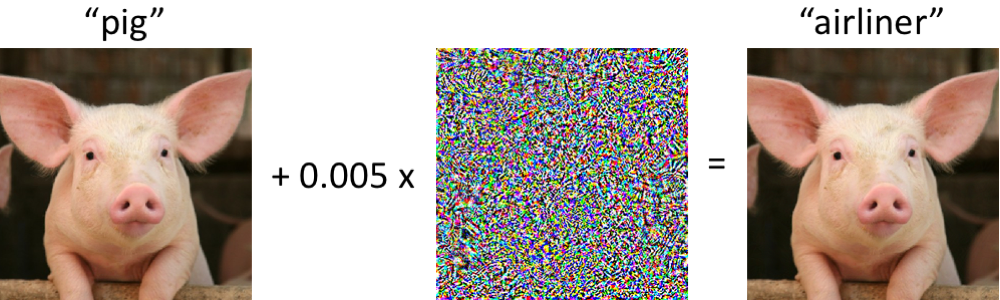
\includegraphics[scale=0.4]{figures/piggie.png}
  \caption{Hyökkäys lentoyhtiötä kohtaan. \citep{adversexamples}}
\end{figure}

Vastakkaishyökkäysten motiivit muovautuvat siis ajan myötä ja kasvattavat tahtomattaan näin hyökkäystaksonomiaa. 

Hyökkäystaksonomia laajentuu tulevaisuudessa eri formaatteihin. Koneoppimisen kukoistaessa voidaan NLP-malleja soveltaa tiedon ääni -tai videoformaatteihin. Tämä antaa puolestaan mahdollisuuden vastakkaishyökätä kyseiseen koneoppimismallia vastaan. Formaattien sisältäkin löytyy erinäisiä hyökkäysrajapintoja. Esimerkiksi ääniformaateissa käytetään kuhunkin käyttötarkoitukseen sopivaa enkoodausta. Ei siis riitä, että hyökättävää ja puolustettavaa tulee uusien formaattien myötä, sillä formaattien sisälläkin tulee tapahtumaan jatkuvasti huomattavaa kehitystä.

Haavoittuvuuksien löytö ruokkii itse itseään. Ensimmäisten vastakkaishyökkäysten kohdistuessa uuteen tietoformaattiin, syntyy tarve puolustukseen tätä vastaan. Toteutuksesta riippuen puolustusmetodin selvittäminen saattaa avata uusia ovia, jotka hyödyttävät hyökkääjiä. Usein haavoittuvuuden tarkastelu vastakkaishyökkäyksissä avaa enemmän mahdollisuuksia uusille hyökkäyksille kuin vanhojen hyökkäysten puolustuksille. Tämä näkyy muun muassa GitHub-repositoriossa \textit{Must-read Papers on Textual Adversarial Attack and Defense (TAAD)}, jossa hyökkäystutkimusten määrä suhteessa puolustustutkimusten määrään on $75:23$ (kuva 4.2).

\begin{figure}[ht]
  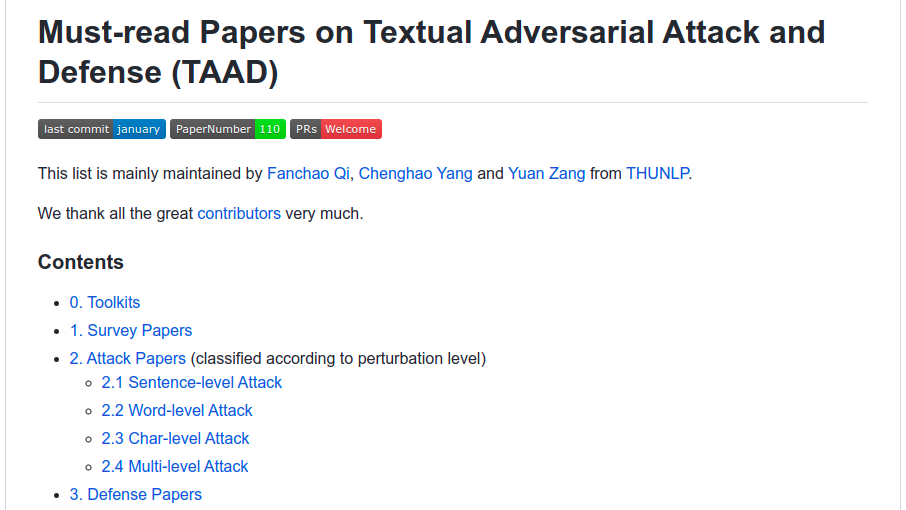
\includegraphics[scale=0.4]{figures/github-papers.png}
  \caption{Hyökkäystutkimusten määrä verrattuna puolustustutkimuksiin.}
\end{figure}